\documentclass[aspectratio=169,10pt]{beamer}

\usetheme{Madrid}
\usecolortheme{seahorse}

\usepackage{amsmath,amssymb,amsfonts}
\usepackage{mathtools}
\usepackage{graphicx}
\usepackage{booktabs}
\usepackage{listings}
\usepackage{xcolor}
\usepackage{bm}
\usepackage{algorithm}
\usepackage{algpseudocode}
\usepackage{tikz}
\usepackage{pgfplots}
\pgfplotsset{compat=1.18}

\graphicspath{{figures/}}

% ── Python listing style ────────────────────────────────────────────────────
\definecolor{codebg}{rgb}{0.97,0.97,0.97}
\definecolor{codegreen}{rgb}{0.0,0.5,0.0}
\definecolor{codepurple}{rgb}{0.4,0.0,0.6}
\definecolor{codeblue}{rgb}{0.0,0.3,0.7}

\lstdefinestyle{python}{
  language=Python,
  basicstyle=\ttfamily\scriptsize,
  keywordstyle=\color{codeblue}\bfseries,
  commentstyle=\color{codegreen}\itshape,
  stringstyle=\color{codepurple},
  numbers=left,
  numberstyle=\tiny\color{gray},
  numbersep=5pt,
  frame=single,
  backgroundcolor=\color{codebg},
  showstringspaces=false,
  breaklines=true,
  tabsize=4,
  captionpos=b
}

\setbeamertemplate{footline}[frame number]
\setbeamertemplate{navigation symbols}{}

% ── Title info ──────────────────────────────────────────────────────────────
\title[Chapter 17: Surrogate Models]{Chapter 17: Surrogate Models}
\subtitle{Algorithms for Optimization, 2nd ed.\ (2026) \\ Kochenderfer \& Wheeler}
\author{Lecture Notes}
\date{\today}

% ── Convenience macros ──────────────────────────────────────────────────────
\newcommand{\vx}{\mathbf{x}}
\newcommand{\vy}{\mathbf{y}}
\newcommand{\vw}{\mathbf{w}}
\newcommand{\vb}{\mathbf{b}}
\newcommand{\btheta}{\boldsymbol{\theta}}
\newcommand{\bX}{\mathbf{X}}
\newcommand{\bB}{\mathbf{B}}
\newcommand{\bI}{\mathbf{I}}
\newcommand{\R}{\mathbb{R}}
\newcommand{\hatf}{\hat{f}}
\DeclareMathOperator*{\minimize}{minimize}

% ════════════════════════════════════════════════════════════════════════════
\begin{document}
% ════════════════════════════════════════════════════════════════════════════

\begin{frame}
  \titlepage
\end{frame}

% ── Outline ─────────────────────────────────────────────────────────────────
\begin{frame}{Outline}
  \tableofcontents
\end{frame}

% ════════════════════════════════════════════════════════════════════════════
\section{Introduction: Fitting Surrogate Models}
% ════════════════════════════════════════════════════════════════════════════

\begin{frame}{Why Surrogate Models?}
  \begin{columns}[T]
    \begin{column}{0.55\textwidth}
      \begin{itemize}
        \item Many real-world objective functions are \alert{expensive} to evaluate
              (e.g.\ CFD simulations, physical experiments).
        \item A \textbf{surrogate model} $\hatf_{\btheta}$ is a \emph{smooth, cheap}
              approximation fitted to a finite set of evaluations.
        \item The surrogate can then be \emph{optimized in place of} the true function.
        \item Key properties required:
          \begin{itemize}
            \item Inexpensive to evaluate.
            \item Smooth enough to apply gradient-based or Bayesian methods.
            \item Generalises well away from observed design points.
          \end{itemize}
      \end{itemize}
    \end{column}
    \begin{column}{0.42\textwidth}
      \centering
      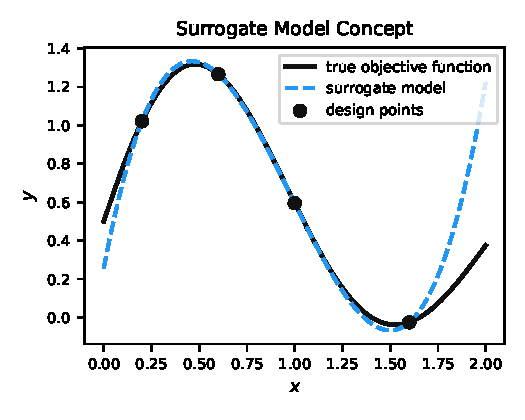
\includegraphics[width=\linewidth]{fig_surrogate_concept}\\[2pt]
      {\scriptsize Surrogate (blue dashed) fitted to design points (dots); deviates from truth far from data.}
    \end{column}
  \end{columns}
\end{frame}

\begin{frame}{Problem Setup}
  \begin{block}{Design Points and Evaluations}
    Suppose we have $m$ design points
    \[
      X = \bigl\{\vx^{(1)}, \vx^{(2)}, \ldots, \vx^{(m)}\bigr\}
      \tag{17.1}
    \]
    and associated objective function evaluations
    \[
      \vy = \bigl\{y^{(1)}, y^{(2)}, \ldots, y^{(m)}\bigr\}
      \tag{17.2}
    \]
  \end{block}

  \begin{block}{Surrogate Predictions}
    For parameter vector $\btheta$, the model predicts
    \[
      \hat{\vy} = \bigl\{\hatf_{\btheta}(\vx^{(1)}),\,
                         \hatf_{\btheta}(\vx^{(2)}),\,
                         \ldots,\,
                         \hatf_{\btheta}(\vx^{(m)})\bigr\}
      \tag{17.3}
    \]
  \end{block}

  \begin{block}{Fitting Objective (Regression)}
    \[
      \minimize_{\btheta} \;\; \|\vy - \hat{\vy}\|_p
      \tag{17.4}
    \]
    \begin{itemize}
      \item $L_2$ norm (MSE): most common, has closed-form solution.
      \item This is called \textbf{regression}.
    \end{itemize}
  \end{block}
\end{frame}

% ════════════════════════════════════════════════════════════════════════════
\section{Linear Models}
% ════════════════════════════════════════════════════════════════════════════

\begin{frame}{Linear Model}
  \begin{block}{Definition (Eq.\ 17.5)}
    \[
      \hatf = w_0 + \vw^{\top}\vx, \qquad
      \btheta = \{w_0,\,\vw\}
    \]
    \begin{itemize}
      \item $w_0 \in \R$: bias (intercept).
      \item $\vw \in \R^n$: weight vector.
      \item For an $n$-dimensional design space: $n+1$ parameters, requires at least $n+1$ samples.
    \end{itemize}
  \end{block}

  \begin{block}{Compact Form (Eq.\ 17.6)}
    Prepend 1 to $\vx$ and absorb $w_0$ into $\btheta = [w_0,\,\vw]$:
    \[
      \hatf = \btheta^{\top}\vx
    \]
  \end{block}

  \begin{block}{Design Matrix (Eq.\ 17.9)}
    \[
      \bX =
      \begin{bmatrix}
        (\vx^{(1)})^{\top} \\
        (\vx^{(2)})^{\top} \\
        \vdots \\
        (\vx^{(m)})^{\top}
      \end{bmatrix}
      \in \R^{m \times (n+1)}
    \]
  \end{block}
\end{frame}

\begin{frame}{Linear Regression: Normal Equations}
  \begin{block}{Optimization Problem (Eq.\ 17.7--17.8)}
    \[
      \minimize_{\btheta} \;\; \|\vy - \hat{\vy}\|_2^2
      \;\equiv\;
      \minimize_{\btheta} \;\; \|\vy - \bX\btheta\|_2^2
    \]
  \end{block}

  \begin{block}{Closed-Form Solution (Eq.\ 17.10)}
    Linear regression has an \alert{analytic solution} via the Moore--Penrose pseudoinverse:
    \[
      \btheta = \bX^{+}\vy
    \]
    where $\bX^{+} = (\bX^{\top}\bX)^{-1}\bX^{\top}$ when $\bX$ has full column rank.
  \end{block}

  \begin{alertblock}{Normal Equation (Exercise 17.1)}
    Setting $\nabla\|\vy - \bX\btheta\|_2^2 = \mathbf{0}$ yields:
    \[
      \bX^{\top}\bX\btheta = \bX^{\top}\vy
    \]
  \end{alertblock}
\end{frame}

\begin{frame}{Linear Regression: Cases}
  \begin{columns}[T]
    \begin{column}{0.50\textwidth}
      \centering
      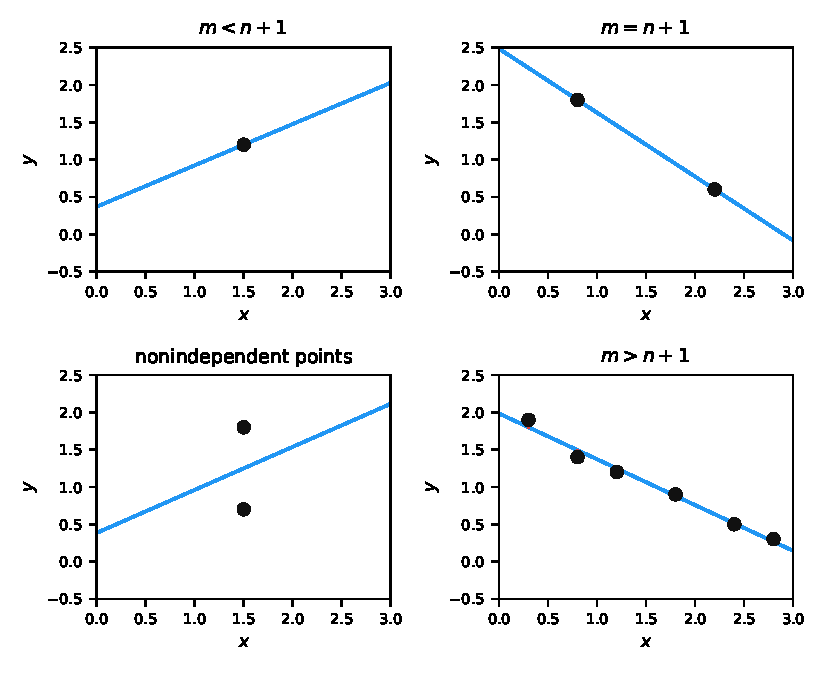
\includegraphics[width=0.92\linewidth]{fig_linear_regression_cases}\\[2pt]
      {\scriptsize Four cases: $m < n{+}1$ (underdetermined), $m = n{+}1$ (exact),
       non-independent, $m > n{+}1$ (overdetermined --- vertical bars show residuals).}
    \end{column}
    \begin{column}{0.47\textwidth}
      \begin{itemize}
        \item $m < n+1$: underdetermined; infinitely many solutions.
          Pseudoinverse gives minimum-norm solution.
        \item $m = n+1$: unique solution (if $\bX$ invertible).
        \item Non-independent: $\bX$ is singular; pseudoinverse still
          gives a unique solution.
        \item $m > n+1$: overdetermined (common case); pseudoinverse
          minimises sum of squared residuals.
      \end{itemize}
      \begin{block}{Key Property}
        The pseudoinverse always returns a \emph{unique} solution
        for any non-empty point configuration.
      \end{block}
    \end{column}
  \end{columns}
\end{frame}

\begin{frame}[fragile]{Linear Regression in Python}
  \begin{columns}[T]
    \begin{column}{0.55\textwidth}
\begin{lstlisting}[style=python, caption={Design matrix and linear regression (Python/NumPy)}]
import numpy as np

def design_matrix(X):
    """X: list of 1-D design points.
    Returns matrix with leading column of ones."""
    m = len(X)
    return np.column_stack([np.ones(m), X])

def linear_regression(X, y):
    """Fit linear model: theta = X^+ y.
    Returns theta = [w0, w1, ..., wn]."""
    Xmat = design_matrix(X)
    # np.linalg.lstsq uses the pseudoinverse
    theta, _, _, _ = np.linalg.lstsq(Xmat, y, rcond=None)
    return theta

# Example: 5 points in 1-D
X = np.array([0.1, 0.4, 0.7, 1.2, 1.8])
y = np.array([0.3, 0.8, 1.2, 1.9, 2.5])
theta = linear_regression(X, y)
print(f"theta = {theta}")
# Prediction at new point
x_new = 1.0
y_pred = theta[0] + theta[1] * x_new
\end{lstlisting}
    \end{column}
    \begin{column}{0.42\textwidth}
      \begin{itemize}
        \item \texttt{np.linalg.lstsq} computes the minimum-norm
              least-squares solution.
        \item Equivalent to $\btheta = \bX^+ \vy$.
        \item \textbf{Numerical example:}\\[3pt]
              $X = [1, 2, 3, 4]$,\; $y = [0, 5, 4, 6]$\\
              Fit polynomial degree $k=1$:
              \[
                \btheta = \begin{bmatrix}-0.5\\1.7\end{bmatrix}
              \]
              so $\hatf(x) = -0.5 + 1.7x$.
      \end{itemize}
    \end{column}
  \end{columns}
\end{frame}

% ════════════════════════════════════════════════════════════════════════════
\section{Basis Functions}
% ════════════════════════════════════════════════════════════════════════════

\begin{frame}{From Linear to Basis-Function Models}
  \begin{block}{Linear Model as Basis Functions (Eq.\ 17.11)}
    \[
      \hatf(\vx) = \theta_1 x_1 + \cdots + \theta_n x_n
                 = \sum_{i=1}^{n} \theta_i x_i
                 = \btheta^{\top}\vx
    \]
    Linear model: basis functions $b_i(\vx) = x_i$.
  \end{block}

  \begin{block}{General Basis-Function Model (Eq.\ 17.12)}
    \[
      \hatf(\vx) = \theta_1 b_1(\vx) + \cdots + \theta_q b_q(\vx)
                 = \sum_{i=1}^{q}\theta_i b_i(\vx)
                 = \btheta^{\top}\vb(\vx)
    \]
    where $b_1, \ldots, b_q$ are arbitrary \emph{basis functions}.
  \end{block}

  \begin{block}{Regression with Basis Functions (Eq.\ 17.13--17.15)}
    \[
      \minimize_{\btheta} \|\vy - \bB\btheta\|_2^2,
      \qquad
      \bB =
      \begin{bmatrix}
        \vb(\vx^{(1)})^{\top} \\
        \vb(\vx^{(2)})^{\top} \\
        \vdots \\
        \vb(\vx^{(m)})^{\top}
      \end{bmatrix},
      \qquad
      \btheta = \bB^{+}\vy
    \]
    \textbf{Any linear combination of basis functions can be fit by regression.}
  \end{block}
\end{frame}

\begin{frame}[fragile]{Basis-Function Regression in Python}
\begin{lstlisting}[style=python, caption={General basis-function regression (Algorithm 17.2 equivalent)}]
import numpy as np

def regression(X, y, bases, lam=0.0):
    """
    Fit surrogate model using basis functions.
    X     : array of m design points
    y     : array of m objective values
    bases : list of q callable basis functions b_i(x)
    lam   : L2 regularisation parameter (default 0)
    Returns: callable model(x)
    """
    B = np.array([[b(x) for b in bases] for x in X])  # m x q
    if lam == 0.0:
        theta, _, _, _ = np.linalg.lstsq(B, y, rcond=None)
    else:
        # theta = (B'B + lam*I)^{-1} B'y
        A = B.T @ B + lam * np.eye(len(bases))
        theta = np.linalg.solve(A, B.T @ y)
    return lambda x: sum(theta[i] * bases[i](x) for i in range(len(theta)))
\end{lstlisting}
  \vspace{-4pt}
  \begin{itemize}
    \item The basis matrix $\bB \in \R^{m \times q}$ replaces the design matrix $\bX$.
    \item Same pseudoinverse solve; $O(mq^2)$ complexity.
    \item \texttt{lam} adds $L_2$ regularisation (see Section 17.4).
  \end{itemize}
\end{frame}

% ────────────────────────────────────────────────────────────────────────────
\subsection{Polynomial Basis Functions}
% ────────────────────────────────────────────────────────────────────────────

\begin{frame}{Polynomial Basis Functions}
  \begin{block}{1-D Polynomial Model of Degree $k$ (Eq.\ 17.16)}
    \[
      \hatf(x) = \theta_0 + \theta_1 x + \theta_2 x^2 + \cdots + \theta_k x^k
               = \sum_{i=0}^{k}\theta_i x^i
    \]
    Basis functions: $b_i(x) = x^i$ for $i = 0, 1, \ldots, k$.
  \end{block}

  \begin{block}{2-D Polynomial of Degree $k$ (Eq.\ 17.17)}
    \[
      b_{ij}(\vx) = x_1^i x_2^j, \quad i,j \in \{0,\ldots,k\},\; i+j \le k
    \]
    \begin{itemize}
      \item Number of basis functions: $\binom{n+k}{k}$ for $n$-dimensional input.
      \item Total parameters for $n=2, k=2$: 6 (constant, $x_1$, $x_2$, $x_1^2$, $x_1 x_2$, $x_2^2$).
    \end{itemize}
  \end{block}

  \begin{exampleblock}{Key Insight}
    A polynomial model is \emph{linear in the higher-dimensional feature space}.
    Fitting reduces to standard linear regression on features $\{x^i\}$.
  \end{exampleblock}
\end{frame}

\begin{frame}[fragile]{Polynomial Regression: Higher-Dimensional View}
  \begin{columns}[T]
    \begin{column}{0.52\textwidth}
      \centering
      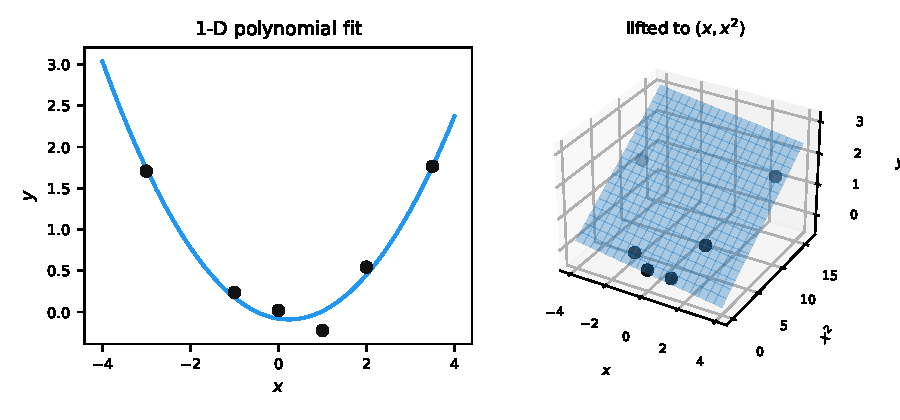
\includegraphics[width=0.95\linewidth]{fig_polynomial_higher_dim}\\[2pt]
      {\scriptsize Left: polynomial fit in 1-D. Right: the same fit is a hyperplane
       in the lifted space $(x,\,x^2)$.}
    \end{column}
    \begin{column}{0.45\textwidth}
      \begin{itemize}
        \item A degree-$k$ polynomial in $\R^n$ is \alert{linear} in $\R^{k+1}$.
        \item Taylor's theorem: any smooth function can be \emph{closely approximated}
              by a polynomial of sufficient degree.
        \item Pitfall: high-degree polynomials can \textbf{overfit} in sparse regions.
      \end{itemize}
\begin{lstlisting}[style=python, basicstyle=\ttfamily\tiny]
# 1-D polynomial bases up to degree k
def poly_bases_1d(k):
    return [lambda x, p=p: x**p
            for p in range(k+1)]

# Example: degree-2 fit
bases = poly_bases_1d(2)
X = np.array([-2, -1, 0, 1, 2])
y = np.array([4.1, 1.0, 0.1, 0.9, 4.0])
model = regression(X, y, bases)
\end{lstlisting}
    \end{column}
  \end{columns}
\end{frame}

% ────────────────────────────────────────────────────────────────────────────
\subsection{Sinusoidal Basis Functions}
% ────────────────────────────────────────────────────────────────────────────

\begin{frame}{Sinusoidal / Fourier Basis Functions}
  \begin{columns}[T]
    \begin{column}{0.50\textwidth}
      \begin{block}{Fourier Series (Eq.\ 17.18--17.20)}
        Any integrable univariate function $f$ on interval $[a,b]$ can be represented as:
        \[
          f(x) = \frac{a_0}{2} + \sum_{k=1}^{\infty}
                 \Bigl[a_k \cos\!\bigl(2\pi k x\bigr)
                       + b_k \sin\!\bigl(2\pi k x\bigr)\Bigr]
        \]
        where
        \[
          a_k = \frac{2}{b-a}\int_a^b f(x)\cos(2\pi k x)\,dx
        \]
        \[
          b_k = \frac{2}{b-a}\int_a^b f(x)\sin(2\pi k x)\,dx
        \]
      \end{block}
      Truncating to $K$ terms gives a surrogate with $2K+1$ parameters.
    \end{column}
    \begin{column}{0.47\textwidth}
      \centering
      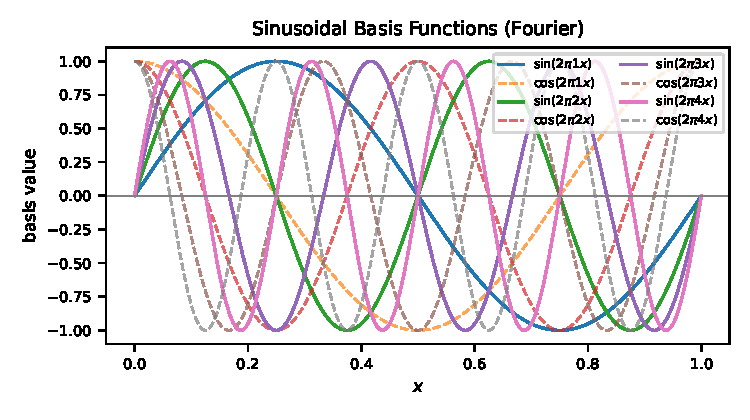
\includegraphics[width=\linewidth]{fig_sinusoidal_bases}\\[2pt]
      {\scriptsize Sinusoidal basis functions for $k=1,2,3,4$.}
      \vspace{4pt}
      \begin{itemize}
        \item Useful when the objective has \emph{periodic} or oscillatory structure.
        \item Can combine with polynomial bases.
        \item Exact representation for periodic functions (complete basis over $L^2$).
      \end{itemize}
    \end{column}
  \end{columns}
\end{frame}

% ────────────────────────────────────────────────────────────────────────────
\subsection{Radial Basis Functions}
% ────────────────────────────────────────────────────────────────────────────

\begin{frame}{Radial Basis Functions (RBF)}
  \begin{block}{Definition}
    A \textbf{radial basis function} (RBF) depends only on the distance
    $r = \|\vx - \mathbf{c}\|$ from a centre $\mathbf{c}$:
    \[
      b(\vx) = \psi\!\bigl(\|\vx - \mathbf{c}\|\bigr)
    \]
  \end{block}

  \begin{columns}[T]
    \begin{column}{0.52\textwidth}
      \centering
      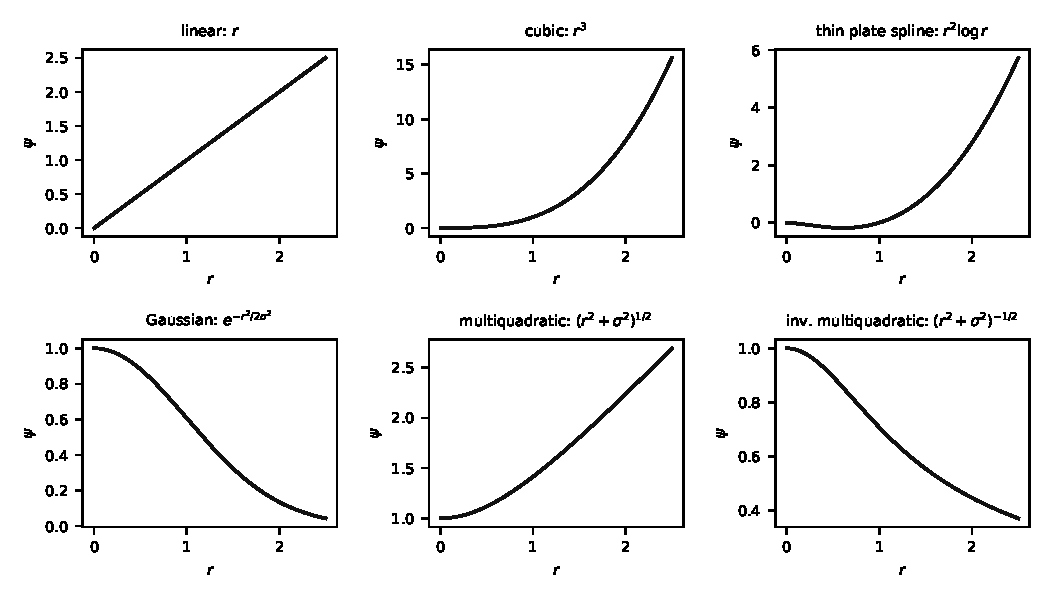
\includegraphics[width=0.95\linewidth]{fig_radial_basis_functions}\\[2pt]
      {\scriptsize Common RBF kernels as a function of radius $r$.}
    \end{column}
    \begin{column}{0.45\textwidth}
      \vspace{4pt}
      \renewcommand{\arraystretch}{1.25}
      \begin{tabular}{ll}
        \toprule
        Name & $\psi(r)$ \\
        \midrule
        Linear & $r$ \\
        Cubic  & $r^3$ \\
        Thin plate spline & $r^2\log r$ \\
        Gaussian & $e^{-r^2/2\sigma^2}$ \\
        Multiquadratic & $(r^2+\sigma^2)^{1/2}$ \\
        Inv.\ multiquadratic & $(r^2+\sigma^2)^{-1/2}$ \\
        \bottomrule
      \end{tabular}
    \end{column}
  \end{columns}
\end{frame}

\begin{frame}[fragile]{RBF Surrogate Construction}
  \begin{block}{RBF Model with $m$ Design Points as Centres}
    Place one RBF at each design point $\vx^{(i)}$:
    \[
      \hatf(\vx) = \sum_{i=1}^{m} \theta_i\,\psi\!\bigl(\|\vx - \vx^{(i)}\|\bigr)
    \]
    The $m\times m$ basis matrix $\bB$ has entries $B_{ij} = \psi(\|\vx^{(i)} - \vx^{(j)}\|)$.
  \end{block}

  \begin{columns}[T]
    \begin{column}{0.50\textwidth}
      \centering
      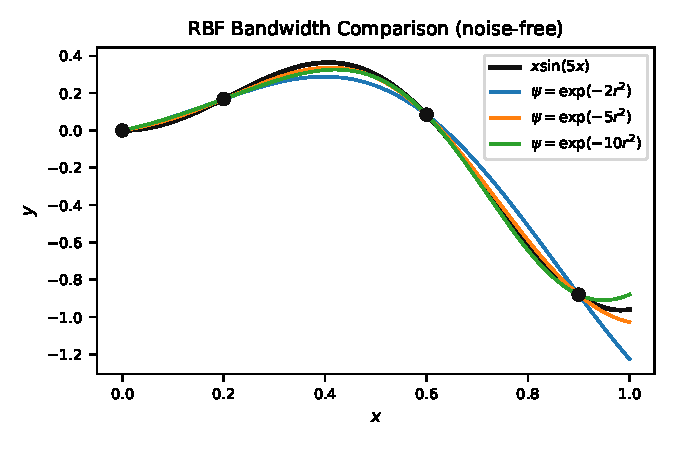
\includegraphics[width=\linewidth]{fig_rbf_bandwidth_comparison}\\[2pt]
      {\scriptsize Gaussian RBFs with different bandwidths fitting $x\sin(5x)$ noise-free.}
    \end{column}
    \begin{column}{0.47\textwidth}
\begin{lstlisting}[style=python, basicstyle=\ttfamily\tiny]
# Gaussian RBF bases centred at design points
def make_rbf_bases(X_train, c=5.0):
    return [lambda x, xi=xi:
            np.exp(-c*(x-xi)**2)
            for xi in X_train]

# Fit
bases = make_rbf_bases(X_train)
model = regression(X_train, y_train,
                   bases, lam=0.0)
\end{lstlisting}
      \begin{itemize}
        \item Bandwidth $c$ controls locality.
        \item Large $c$: narrow, interpolates tightly.
        \item Small $c$: wide, smoother extrapolation.
        \item Choose $c$ via cross-validation (Sec.\ 17.5).
      \end{itemize}
    \end{column}
  \end{columns}
\end{frame}

% ════════════════════════════════════════════════════════════════════════════
\section{Fitting Noisy Objective Functions}
% ════════════════════════════════════════════════════════════════════════════

\begin{frame}{Noisy Observations and $L_2$ Regularisation}
  \begin{block}{Problem}
    When objective evaluations are \alert{noisy}: $y^{(i)} = f(\vx^{(i)}) + \epsilon^{(i)}$,
    an unregularised surrogate may \textbf{overfit} the noise.
  \end{block}

  \begin{block}{Regularised Regression ($L_2$ / Ridge, Eq.\ 17.24)}
    Add a penalty on parameter magnitude:
    \[
      \minimize_{\btheta} \;\;
      \|\vy - \bB\btheta\|_2^2 + \lambda\|\btheta\|_2^2
    \]
    \begin{itemize}
      \item $\lambda \geq 0$: \emph{smoothing parameter} (hyperparameter).
      \item $\lambda = 0$: no regularisation (standard regression).
    \end{itemize}
  \end{block}

  \begin{block}{Closed-Form Solution (Eq.\ 17.25)}
    \[
      \btheta = \bigl(\bB^{\top}\bB + \lambda\bI\bigr)^{-1}\bB^{\top}\vy
    \]
    \begin{itemize}
      \item $(\bB^{\top}\bB + \lambda\bI)$ is always \emph{invertible} for $\lambda > 0$.
      \item Viewable as adding a fictitious prior $\btheta \sim \mathcal{N}(\mathbf{0}, \sigma^2/\lambda\,\bI)$.
    \end{itemize}
  \end{block}
\end{frame}

\begin{frame}[fragile]{Effect of Regularisation}
  \begin{columns}[T]
    \begin{column}{0.52\textwidth}
      \centering
      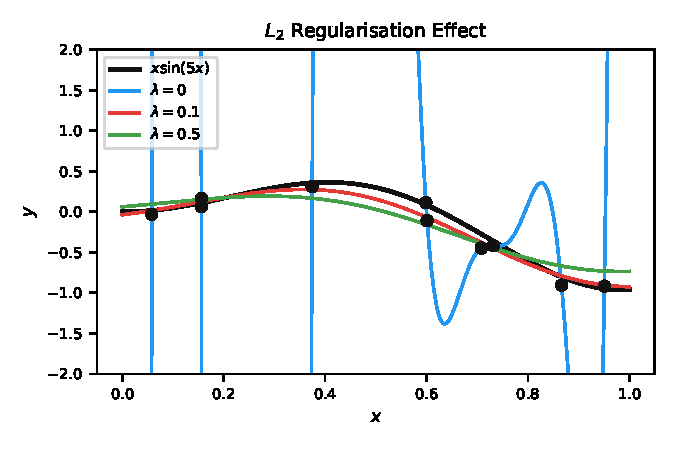
\includegraphics[width=\linewidth]{fig_regularisation}\\[2pt]
      {\scriptsize 10 noisy samples of $x\sin(5x)$. Large $\lambda$ over-smooths;
       $\lambda=0$ overfits. Cross-validation finds optimal $\lambda\approx 0.1$.}
    \end{column}
    \begin{column}{0.45\textwidth}
\begin{lstlisting}[style=python, basicstyle=\ttfamily\tiny, caption={Regularised RBF regression}]
import numpy as np

def regression_regularised(X, y, bases, lam):
    """Ridge regression with L2 penalty lam."""
    B = np.array([[b(x) for b in bases]
                  for x in X])      # m x q
    A = B.T @ B + lam * np.eye(len(bases))
    theta = np.linalg.solve(A, B.T @ y)
    return lambda x: sum(theta[i]*bases[i](x)
                         for i in range(len(theta)))

# Fit with lambda=0.1
X = np.linspace(0, 1, 10)
y = X*np.sin(5*X) + 0.1*np.random.randn(10)
bases = make_rbf_bases(X, c=5.0)
model = regression_regularised(X, y, bases,
                                lam=0.1)
\end{lstlisting}
      \begin{itemize}
        \item \textbf{Bias--variance trade-off:}
          small $\lambda$ = low bias, high variance;
          large $\lambda$ = high bias, low variance.
        \item Optimal $\lambda$ selected by cross-validation.
      \end{itemize}
    \end{column}
  \end{columns}
\end{frame}

% ════════════════════════════════════════════════════════════════════════════
\section{Model Selection}
% ════════════════════════════════════════════════════════════════════════════

\begin{frame}{Model Selection: The Bias--Variance Trade-off}
  \begin{columns}[T]
    \begin{column}{0.50\textwidth}
      \centering
      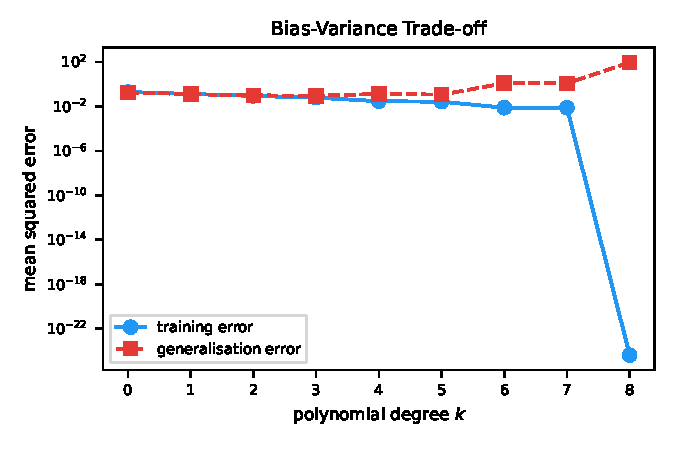
\includegraphics[width=\linewidth]{fig_bias_variance}\\[2pt]
      {\scriptsize Training error decreases monotonically with polynomial degree.
        Generalisation error is U-shaped.}
    \end{column}
    \begin{column}{0.47\textwidth}
      \begin{itemize}
        \item \textbf{Underfitting (high bias):} Model too simple,
              misses important trends.
        \item \textbf{Overfitting (high variance):} Model too complex,
              fits noise, poor generalisation.
        \item \textbf{Generalisation error:}
          \[
            \epsilon_{\text{gen}} = \mathbb{E}\bigl[(y - \hatf(\vx))^2\bigr]
          \]
        \item True generalisation error is \emph{unknowable} exactly ---
              we use empirical estimates.
      \end{itemize}
      \begin{block}{Example 17.1}
        $f(x) = x/10 + \sin(x)/4 + e^{-x^2}$\\
        9 points in $[-4,4]$; evaluated on $[-5,5]$.\\
        Optimal degree $\approx 3$.
      \end{block}
    \end{column}
  \end{columns}
\end{frame}

\begin{frame}{Polynomial Degree: Training vs Generalisation}
  \centering
  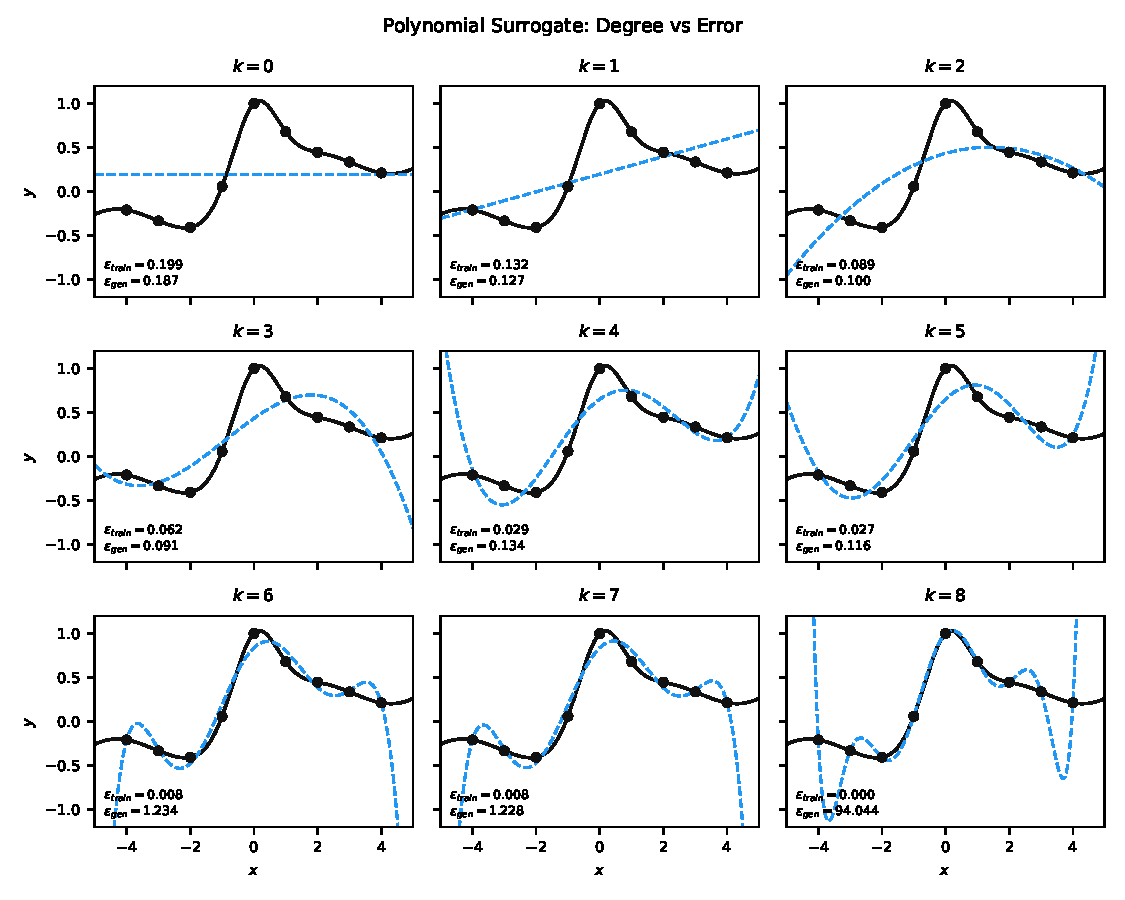
\includegraphics[width=0.80\linewidth]{fig_poly_degree_comparison}\\[2pt]
  {\scriptsize $f(x)=x/10+\sin(x)/4+e^{-x^2}$ (black), polynomial fit (blue dashed).
   Degrees $k=0$--$8$: $k=3$ minimises generalisation error.}
\end{frame}

% ────────────────────────────────────────────────────────────────────────────
\subsection{Holdout Method}
% ────────────────────────────────────────────────────────────────────────────

\begin{frame}[fragile]{Model Selection: Holdout Method}
  \begin{columns}[T]
    \begin{column}{0.48\textwidth}
      \centering
      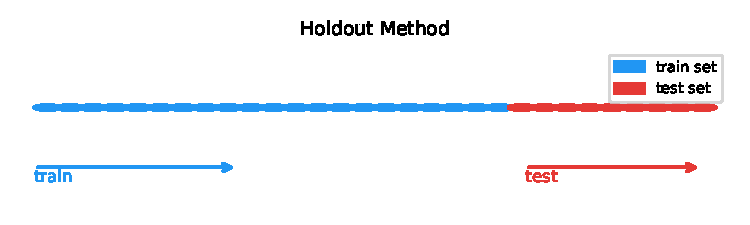
\includegraphics[width=\linewidth]{fig_holdout_schematic}\\[2pt]
      {\scriptsize Split dataset into train (blue) and test (red).}

      \vspace{6pt}
      \begin{block}{Procedure}
        \begin{enumerate}
          \item Split $m$ samples: $S_{\text{train}}$ ($\sim$70--80\%) and $S_{\text{test}}$.
          \item Fit model on $S_{\text{train}}$.
          \item Evaluate on $S_{\text{test}}$ to estimate $\epsilon_{\text{gen}}$.
        \end{enumerate}
      \end{block}
    \end{column}
    \begin{column}{0.49\textwidth}
\begin{lstlisting}[style=python, basicstyle=\ttfamily\tiny, caption={Holdout method (Algorithm 17.7)}]
import numpy as np

def holdout_split(m, frac=0.7, seed=0):
    """Returns (train_idx, test_idx)."""
    rng = np.random.default_rng(seed)
    perm = rng.permutation(m)
    n_train = int(frac * m)
    return perm[:n_train], perm[n_train:]

def holdout_estimate(X, y, bases, seed=0):
    tr, te = holdout_split(len(X), seed=seed)
    model = regression(X[tr], y[tr], bases)
    preds = np.array([model(x) for x in X[te]])
    return np.mean((y[te] - preds)**2)
\end{lstlisting}
      \begin{itemize}
        \item Simple and fast.
        \item \textbf{Drawback:} result depends on which samples fall in test set.
        \item Solution: average over multiple random splits (cross-validation).
      \end{itemize}
    \end{column}
  \end{columns}
\end{frame}

% ────────────────────────────────────────────────────────────────────────────
\subsection{Cross-Validation}
% ────────────────────────────────────────────────────────────────────────────

\begin{frame}[fragile]{$k$-Fold Cross-Validation}
  \begin{columns}[T]
    \begin{column}{0.46\textwidth}
      \centering
      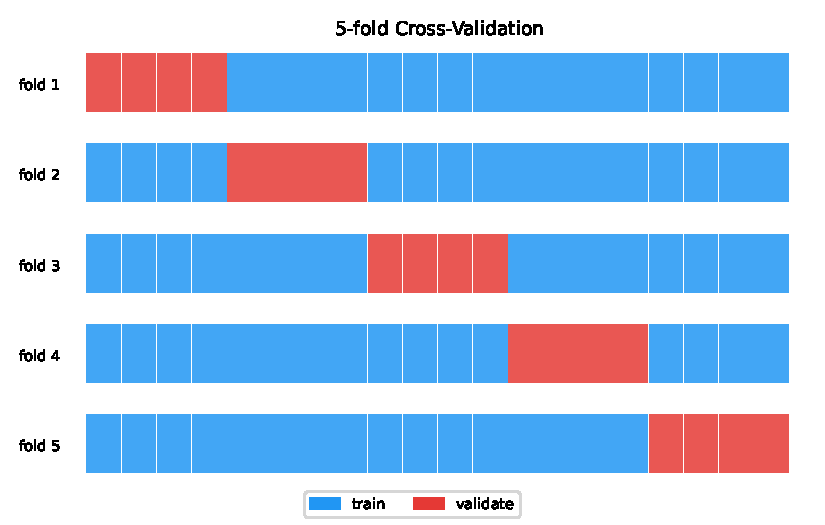
\includegraphics[width=\linewidth]{fig_kfold_schematic}\\[2pt]
      {\scriptsize 5-fold CV: each fold takes a turn as the validation set.}
    \end{column}
    \begin{column}{0.51\textwidth}
      \begin{block}{Algorithm (Alg.\ 17.10)}
        \begin{enumerate}
          \item Partition $m$ samples into $k$ folds.
          \item For $i = 1, \ldots, k$:
            \begin{itemize}
              \item Train on all folds except fold $i$.
              \item Validate on fold $i$.
            \end{itemize}
          \item Estimate $\epsilon_{\text{gen}} = \frac{1}{k}\sum_{i=1}^{k}\epsilon_{\text{test}}^{(i)}$.
        \end{enumerate}
      \end{block}
      \begin{itemize}
        \item Uses \emph{all} data for both training and validation.
        \item \textbf{Leave-one-out CV} ($k = m$): deterministic, trains $m$ models.
        \item Common choices: $k = 5$ or $k = 10$.
      \end{itemize}
      \begin{block}{Complexity}
        Trains $k$ models, each on $(k-1)/k$ fraction of data.
        Total cost: $O(k \cdot \text{fit cost})$.
      \end{block}
    \end{column}
  \end{columns}
\end{frame}

\begin{frame}[fragile]{Cross-Validation in Python}
\begin{lstlisting}[style=python, caption={k-fold cross-validation (Algorithm 17.10 equivalent)}]
import numpy as np
from dataclasses import dataclass
from typing import List

@dataclass
class TrainTest:
    train: np.ndarray
    test:  np.ndarray

def k_fold_cv_sets(m: int, k: int) -> List[TrainTest]:
    """Generate k train/test index splits."""
    perm = np.random.permutation(m)
    fold_size = m // k
    sets = []
    for i in range(k):
        test_idx  = perm[i*fold_size:(i+1)*fold_size]
        train_idx = np.concatenate([perm[:i*fold_size],
                                    perm[(i+1)*fold_size:]])
        sets.append(TrainTest(train_idx, test_idx))
    return sets

def cv_estimate(X, y, sets, bases, lam=0.0):
    """Mean CV error across all folds."""
    errors = []
    for s in sets:
        model = regression(X[s.train], y[s.train], bases, lam)
        preds = np.array([model(x) for x in X[s.test]])
        errors.append(np.mean((y[s.test] - preds)**2))
    return np.mean(errors)
\end{lstlisting}
\end{frame}

\begin{frame}[fragile]{Cross-Validation for Hyperparameter Selection (Example 17.2)}
  \begin{columns}[T]
    \begin{column}{0.45\textwidth}
      \centering
      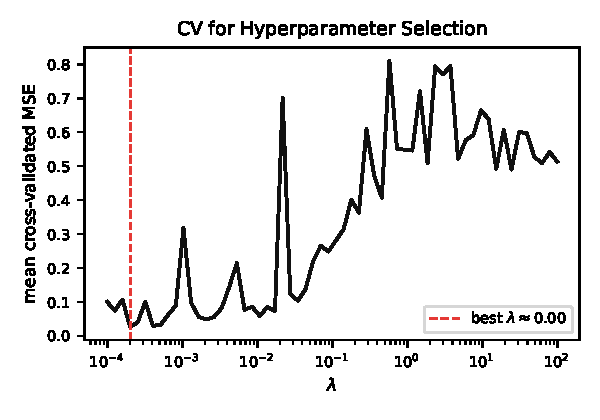
\includegraphics[width=\linewidth]{fig_cv_lambda}\\[2pt]
      {\scriptsize Mean cross-validated MSE vs.\ $\lambda$ for 10 noisy samples of
        $f(x) = \sin(2x)\cos(10x) + \epsilon/10$.
        Minimum near $\lambda \approx 0.2$.}
    \end{column}
    \begin{column}{0.52\textwidth}
\begin{lstlisting}[style=python, basicstyle=\ttfamily\tiny]
import numpy as np

np.random.seed(0)
m = 10
X = np.random.rand(m)
y = np.sin(2*X)*np.cos(10*X) + np.random.randn(m)/10

# Gaussian RBF basis
c = 5.0
bases = [lambda x, xi=xi: np.exp(-c*(x-xi)**2)
         for xi in X]

# 3-fold CV over lambda grid
sets = k_fold_cv_sets(m, k=3)
lambdas = np.logspace(-4, 2, 60)
cv_errs = [cv_estimate(X, y, sets, bases, lam)
           for lam in lambdas]

best_lam = lambdas[np.argmin(cv_errs)]
print(f"Best lambda = {best_lam:.4f}")
\end{lstlisting}
      \begin{itemize}
        \item Sweep $\lambda$ over logarithmic grid.
        \item Select model minimising CV error.
        \item Result: $\lambda_{\text{best}} \approx 0.2$.
      \end{itemize}
    \end{column}
  \end{columns}
\end{frame}

% ────────────────────────────────────────────────────────────────────────────
\subsection{Bootstrap}
% ────────────────────────────────────────────────────────────────────────────

\begin{frame}[fragile]{The Bootstrap Method}
  \begin{columns}[T]
    \begin{column}{0.46\textwidth}
      \centering
      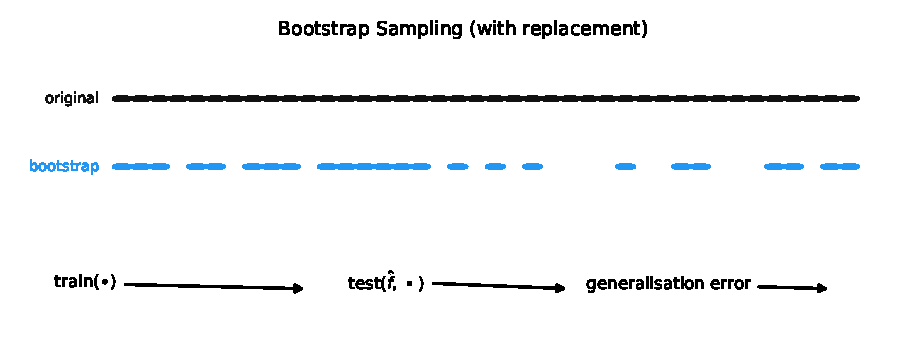
\includegraphics[width=0.92\linewidth]{fig_bootstrap_schematic}\\[2pt]
      {\scriptsize Bootstrap: sample $m$ indices \emph{with replacement}, train on
       bootstrap sample, test on full dataset.}
    \end{column}
    \begin{column}{0.51\textwidth}
      \begin{block}{Bootstrap Error Estimate (Eq.\ 17.31--17.32)}
        If $b$ bootstrap samples are used:
        \[
          \epsilon_{\text{boot}} = \frac{1}{b}\sum_{i=1}^{b}\epsilon_{\text{test}}^{(i)}
          = \frac{1}{m}\sum_{j=1}^{m}\frac{1}{b}\sum_{i=1}^{b}
            \bigl(y^{(j)} - \hatf^{(i)}(\vx^{(j)})\bigr)^2
        \]
      \end{block}
      \begin{block}{Leave-One-Out Bootstrap (Eq.\ 17.33)}
        \[
          \epsilon_{\text{loo-boot}} = \frac{1}{m}\sum_{j=1}^{m}
          \frac{1}{c_{-j}}\sum_{\substack{i=1 \\ j \notin S^{(i)}}}^{b}
          \bigl(y^{(j)} - \hatf^{(i)}(\vx^{(j)})\bigr)^2
        \]
        where $c_{-j}$ = number of bootstrap samples not containing $j$.
      \end{block}
      \begin{itemize}
        \item Expected fraction of \emph{out-of-bag} samples: $1 - e^{-1} \approx 0.632$.
      \end{itemize}
    \end{column}
  \end{columns}
\end{frame}

\begin{frame}[fragile]{Bootstrap in Python}
\begin{lstlisting}[style=python, caption={Bootstrap error estimation (Algorithm 17.12/17.13 equivalent)}]
import numpy as np

def bootstrap_sets(m: int, b: int):
    """Generate b bootstrap (train, test=all) pairs."""
    return [(np.random.choice(m, m, replace=True),
             np.arange(m)) for _ in range(b)]

def bootstrap_estimate(X, y, b_sets, bases, lam=0.0):
    """Bootstrap generalisation error estimate."""
    errors = []
    for train, test in b_sets:
        model = regression(X[train], y[train], bases, lam)
        preds = np.array([model(x) for x in X[test]])
        errors.append(np.mean((y[test] - preds)**2))
    return np.mean(errors)

def loo_bootstrap_estimate(X, y, b_sets, bases, lam=0.0):
    """Leave-one-out bootstrap estimate."""
    m = len(X)
    models = [regression(X[tr], y[tr], bases, lam)
              for tr, _ in b_sets]
    eps = 0.0
    for j in range(m):
        c_j = sum(1 for i,(tr,_) in enumerate(b_sets)
                  if j not in tr)
        if c_j == 0:
            continue
        delta = sum((y[j] - models[i](X[j]))**2
                    for i,(tr,_) in enumerate(b_sets)
                    if j not in tr)
        eps += delta / c_j
    return eps / m
\end{lstlisting}
\end{frame}

% ────────────────────────────────────────────────────────────────────────────
\subsection{AIC and BIC}
% ────────────────────────────────────────────────────────────────────────────

\begin{frame}{Information-Theoretic Model Selection: AIC and BIC}
  \begin{block}{Akaike Information Criterion (AIC)}
    \[
      \mathrm{AIC} = 2q - 2\ln\hat{\mathcal{L}}
    \]
    \begin{itemize}
      \item $q$: number of model parameters.
      \item $\hat{\mathcal{L}}$: maximum likelihood.
      \item For Gaussian noise: $\mathrm{AIC} = n\ln(\mathrm{SSE}/n) + 2q$.
      \item Penalises complexity mildly.
    \end{itemize}
  \end{block}

  \begin{block}{Bayesian Information Criterion (BIC)}
    \[
      \mathrm{BIC} = q\ln n - 2\ln\hat{\mathcal{L}}
    \]
    \begin{itemize}
      \item Penalises complexity more heavily than AIC (factor $\ln n$ vs 2).
      \item Tends to select \emph{sparser} models.
    \end{itemize}
  \end{block}

  \begin{columns}[T]
    \begin{column}{0.50\textwidth}
      \centering
      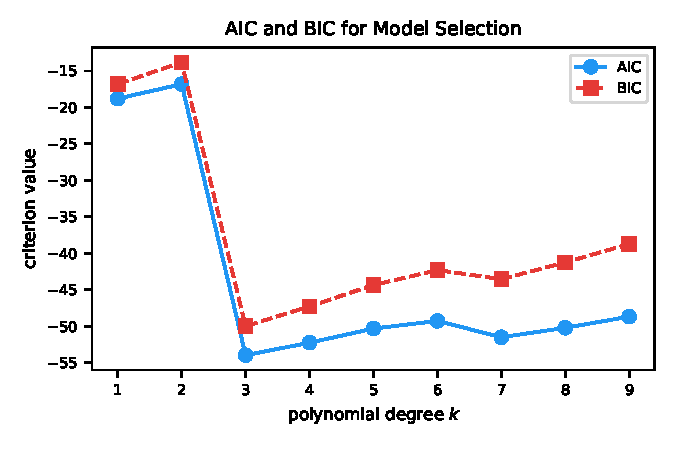
\includegraphics[width=0.9\linewidth]{fig_aic_bic}
    \end{column}
    \begin{column}{0.47\textwidth}
      \begin{itemize}
        \item Both AIC and BIC balance \emph{fit quality} vs.\ \emph{complexity}.
        \item Do \emph{not} require a held-out validation set.
        \item Select the model with the \alert{lowest} AIC or BIC.
      \end{itemize}
    \end{column}
  \end{columns}
\end{frame}

% ════════════════════════════════════════════════════════════════════════════
\section{Multifidelity Surrogate Models}
% ════════════════════════════════════════════════════════════════════════════

\begin{frame}{Multifidelity Surrogate Models}
  \begin{block}{Motivation}
    Often multiple evaluation sources are available:
    \begin{itemize}
      \item $f_h$: \textbf{high-fidelity} (expensive, accurate) -- e.g.\ full CFD.
      \item $f_\ell$: \textbf{low-fidelity} (cheap, biased) -- e.g.\ reduced-order model.
    \end{itemize}
    We have many evaluations $X_\ell$ from $f_\ell$ but few from $X_h$.
  \end{block}

  \begin{columns}[T]
    \begin{column}{0.48\textwidth}
      \centering
      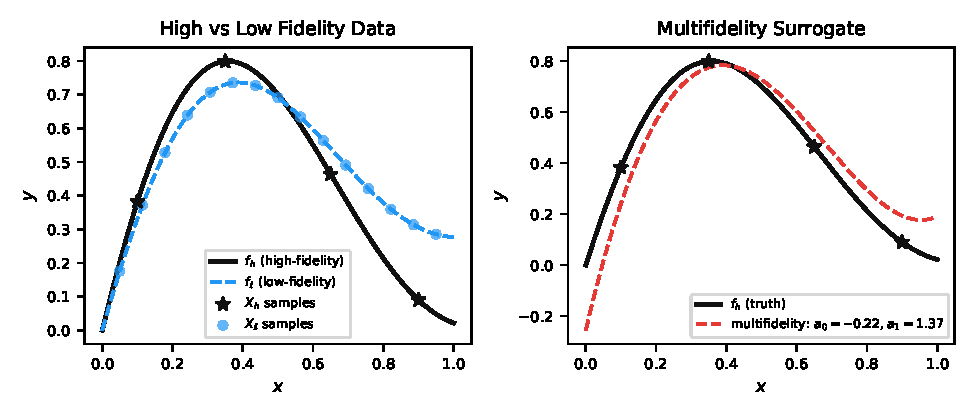
\includegraphics[width=\linewidth]{fig_multifidelity}\\[2pt]
      {\scriptsize Left: high vs low fidelity functions. Right: linear correction
       multifidelity surrogate.}
    \end{column}
    \begin{column}{0.49\textwidth}
      \begin{block}{Linear Multifidelity Model (Eq.\ 17.36)}
        \[
          f_h(\vx) \approx a_0 + a_1\,\hatf_\ell(\vx)
        \]
        \begin{itemize}
          \item $\hatf_\ell$: surrogate fitted to low-fidelity data $X_\ell$.
          \item $a_0, a_1$: correction parameters fitted using $X_h$.
          \item $a_1 \approx$ scaling; $a_0 \approx$ bias correction.
        \end{itemize}
      \end{block}
    \end{column}
  \end{columns}
\end{frame}

\begin{frame}[fragile]{Multifidelity Model: Construction and Python}
  \begin{columns}[T]
    \begin{column}{0.52\textwidth}
\begin{lstlisting}[style=python, basicstyle=\ttfamily\tiny, caption={Linear multifidelity surrogate}]
import numpy as np

def multifidelity_surrogate(X_lo, y_lo,
                             X_hi, y_hi,
                             lo_bases):
    """
    Build multifidelity surrogate.
    Step 1: fit low-fidelity model
    Step 2: use low-fi predictions at X_hi
            to fit linear correction a0, a1
    """
    # Step 1: low-fidelity surrogate
    f_lo = regression(X_lo, y_lo, lo_bases)

    # Step 2: linear correction
    lo_at_hi = np.array([f_lo(x) for x in X_hi])
    A = np.column_stack([np.ones(len(X_hi)),
                         lo_at_hi])
    params, _, _, _ = np.linalg.lstsq(A, y_hi,
                                       rcond=None)
    a0, a1 = params

    # Combined multifidelity model
    def mf_model(x):
        return a0 + a1 * f_lo(x)
    return mf_model, (a0, a1)
\end{lstlisting}
    \end{column}
    \begin{column}{0.45\textwidth}
      \vspace{6pt}
      \begin{block}{Procedure Summary}
        \begin{enumerate}
          \item Fit $\hatf_\ell$ on large $X_\ell$ dataset.
          \item Evaluate $\hatf_\ell(\vx^{(i)})$ at all high-fidelity points $\vx^{(i)} \in X_h$.
          \item Regress $y_h^{(i)}$ against $\hatf_\ell(\vx^{(i)})$ to find $a_0, a_1$.
          \item Final model: $\hatf(\vx) = a_0 + a_1 \hatf_\ell(\vx)$.
        \end{enumerate}
      \end{block}
      \begin{itemize}
        \item Extension: non-hierarchical datasets, Bayesian multifidelity.
        \item Application: aircraft collision avoidance (Exercise 17.5):
          \[
            a_0 \approx 0,\quad a_1 \approx 0.01
          \]
      \end{itemize}
    \end{column}
  \end{columns}
\end{frame}

\begin{frame}{Multifidelity: Cases and Considerations}
  \begin{block}{Case 1: Hierarchical (most common)}
    $f_h$ and $f_\ell$ measure the \emph{same} quantity at different accuracy levels.
    \begin{itemize}
      \item Low fidelity is a fast approximation (coarser mesh, fewer Monte Carlo samples).
      \item Linear correction typically adequate.
    \end{itemize}
  \end{block}

  \begin{block}{Case 2: Non-comparable outputs}
    $f_\ell$ and $f_h$ measure \emph{related but different} quantities.
    \begin{itemize}
      \item Example: $f_\ell$ = sweetness/salinity proxy; $f_h$ = customer satisfaction.
      \item Build a \emph{mapping} between outputs using shared design samples.
    \end{itemize}
  \end{block}

  \begin{block}{Case 3: Non-hierarchical datasets}
    Multiple sources of unknown or variable fidelity.
    \begin{itemize}
      \item Build separate surrogates for each source.
      \item Combine predictions (weighted averaging, Bayesian model averaging).
    \end{itemize}
  \end{block}
\end{frame}

% ════════════════════════════════════════════════════════════════════════════
\section{Summary \& Exercises}
% ════════════════════════════════════════════════════════════════════════════

\begin{frame}{Chapter 17 Summary}
  \begin{block}{Key Takeaways}
    \begin{enumerate}
      \item \textbf{Surrogate models} approximate expensive objective functions
            using cheap, smooth models fitted by regression.
      \item \textbf{Regression} minimises $\|\vy - \bB\btheta\|_2^2$;
            analytic solution $\btheta = \bB^+\vy$.
      \item \textbf{Basis functions} extend linear models to nonlinear surrogates:
            polynomial, sinusoidal (Fourier), radial (RBF).
      \item \textbf{Noisy objectives}: $L_2$ regularisation ($\lambda > 0$) prevents
            overfitting; optimal $\lambda$ via cross-validation.
      \item \textbf{Model selection} balances bias (underfitting) and variance (overfitting)
            using holdout, $k$-fold CV, bootstrap, AIC, or BIC.
      \item \textbf{Multifidelity} surrogates exploit cheap low-fidelity data to
            boost accuracy with few expensive high-fidelity evaluations.
    \end{enumerate}
  \end{block}

  \begin{columns}[T]
    \begin{column}{0.48\textwidth}
      \begin{alertblock}{Practical Guidelines}
        \begin{itemize}
          \item Start with linear or low-degree polynomial.
          \item Switch to RBF for complex nonlinearity.
          \item Always use cross-validation for hyperparameter selection.
        \end{itemize}
      \end{alertblock}
    \end{column}
    \begin{column}{0.48\textwidth}
      \begin{exampleblock}{Connections to Other Chapters}
        \begin{itemize}
          \item Chapter 16: sampling plans to build $X$.
          \item Chapter 18: Bayesian optimisation uses GP surrogate.
          \item Chapter 13: pseudoinverse (linear algebra).
          \item Chapter 15: multiobjective (regularisation).
        \end{itemize}
      \end{exampleblock}
    \end{column}
  \end{columns}
\end{frame}

\begin{frame}[allowframebreaks]{Exercises (Chapter 17)}
  \begin{block}{Exercise 17.1 -- Normal Equation}
    Derive an expression satisfied by the optimum of
    $\minimize_{\btheta}\|\vy - \bX\btheta\|_2^2$ by setting the gradient to zero.
    \\[4pt]
    \textbf{Solution:}
    \[
      \nabla_{\btheta}(\vy - \bX\btheta)^{\top}(\vy - \bX\btheta)
      = -2\bX^{\top}(\vy - \bX\btheta) = \mathbf{0}
      \;\implies\;
      \bX^{\top}\bX\btheta = \bX^{\top}\vy
    \]
  \end{block}

  \begin{block}{Exercise 17.2 -- When to Use Complex Models}
    When would we use a more descriptive model (polynomial) versus simpler (linear)?
    \\[4pt]
    \textbf{Solution:} Use more complex models when more data are available.
    With few samples, simpler models with fewer degrees of freedom prevent overfitting.
  \end{block}

  \begin{block}{Exercise 17.3 -- Iterative Solvers for Large Regression}
    Why might we use iterative methods instead of the analytic solution?
    \\[4pt]
    \textbf{Solution:} The design matrix $\bB \in \R^{m \times q}$ can be extremely large.
    The normal equations require $O(q^3)$ factorisation; iterative methods (stochastic
    gradient descent) have $O(q)$ memory and are the only viable option at scale.
  \end{block}

  \framebreak

  \begin{block}{Exercise 17.4 -- Leave-One-Out CV}
    Evaluate $f$ at $x = 1,2,3,4$ giving $y = 0,5,4,6$.
    Compute the LOOCV MSE for polynomial degrees $k = 0,\ldots,4$.
    \\[4pt]
    \textbf{Solution:} LOOCV with $k=4$ folds.
    Minimum MSE achieved at $k=1$ (linear model), giving
    $\btheta \approx [-0.5,\;1.7]$, i.e.\ $\hatf(x) = -0.5 + 1.7x$.
  \end{block}

  \begin{block}{Exercise 17.5 -- Aircraft Collision Avoidance}
    $f_\ell$: 1\,000 flight hours (biased scenarios, 100\% safety-critical).
    $f_h$: 1\,000\,000 flight hours (1\% safety-critical).
    Expected $a_0$ and $a_1$ in $f_h \approx a_0 + a_1 f_\ell$?
    \\[4pt]
    \textbf{Solution:}
    $f_\ell$ overestimates collision rate by $\sim$100$\times$ (all scenarios critical).
    Therefore $a_1 \approx 0.01$ to scale down; $a_0 \approx 0$ (no additive bias needed).
  \end{block}
\end{frame}

\begin{frame}{References}
  \begin{itemize}
    \item M. J. Kochenderfer and T. A. Wheeler,
          \emph{Algorithms for Optimization}, 2nd ed.\ MIT Press, 2026.
          Chapter 17: Surrogate Models (pp.\ 365--388).
    \item K. P. Murphy, \emph{Machine Learning: A Probabilistic Perspective}.
          MIT Press, 2012.
    \item P. Jiang, Q. Zhou, and X. Shao,
          \emph{Surrogate Model-Based Engineering Design and Optimization}.
          Springer, 2020.
    \item A. Forrester, A. Sobester, and A. Keane,
          \emph{Engineering Design via Surrogate Modelling: A Practical Guide}.
          Wiley, 2008.
    \item M. Stone, ``Cross-Validatory Choice and Assessment of Statistical Predictions,''
          \emph{J.\ Royal Statistical Society}, vol.\ 36, no.\ 2, pp.\ 111--147, 1974.
    \item B. Efron, ``Bootstrap Methods: Another Look at the Jackknife,''
          \emph{The Annals of Statistics}, vol.\ 7, pp.\ 1--26, 1979.
  \end{itemize}
\end{frame}

\end{document}
